\documentclass[tikz,border=12pt]{standalone}
\usepackage{tikz}
\usepackage{amsmath,amssymb}
\usepackage{fontawesome5}
\usetikzlibrary{arrows.meta,positioning,fit,backgrounds,calc,shadows,shapes.geometric}

% Color definitions
\definecolor{lavenderDark}{RGB}{15, 44, 89}
\definecolor{lavenderDeep}{RGB}{10, 28, 58}
\definecolor{lavenderMedium}{RGB}{29, 78, 158}
\definecolor{lavenderLight}{RGB}{240, 246, 255}
\definecolor{lavenderBorder}{RGB}{180, 205, 237}
\definecolor{prismNavy}{RGB}{15, 44, 89}
\definecolor{prismBlue}{RGB}{29, 78, 158}
\definecolor{prismTeal}{RGB}{13, 148, 136}
\definecolor{prismGold}{RGB}{217, 119, 6}
\definecolor{prismDark}{RGB}{15, 23, 42}
\definecolor{cInput}{RGB}{241, 245, 249}
\definecolor{cStem}{RGB}{224, 242, 254}
\definecolor{cStage1}{RGB}{209, 250, 229}
\definecolor{cStage2}{RGB}{254, 243, 199}
\definecolor{cStage4}{RGB}{207, 250, 254}
\definecolor{cHead}{RGB}{219, 234, 254}

\begin{document}
% Level-1 Data Flow Diagram (DFD) for Power Grid Visual Analytics
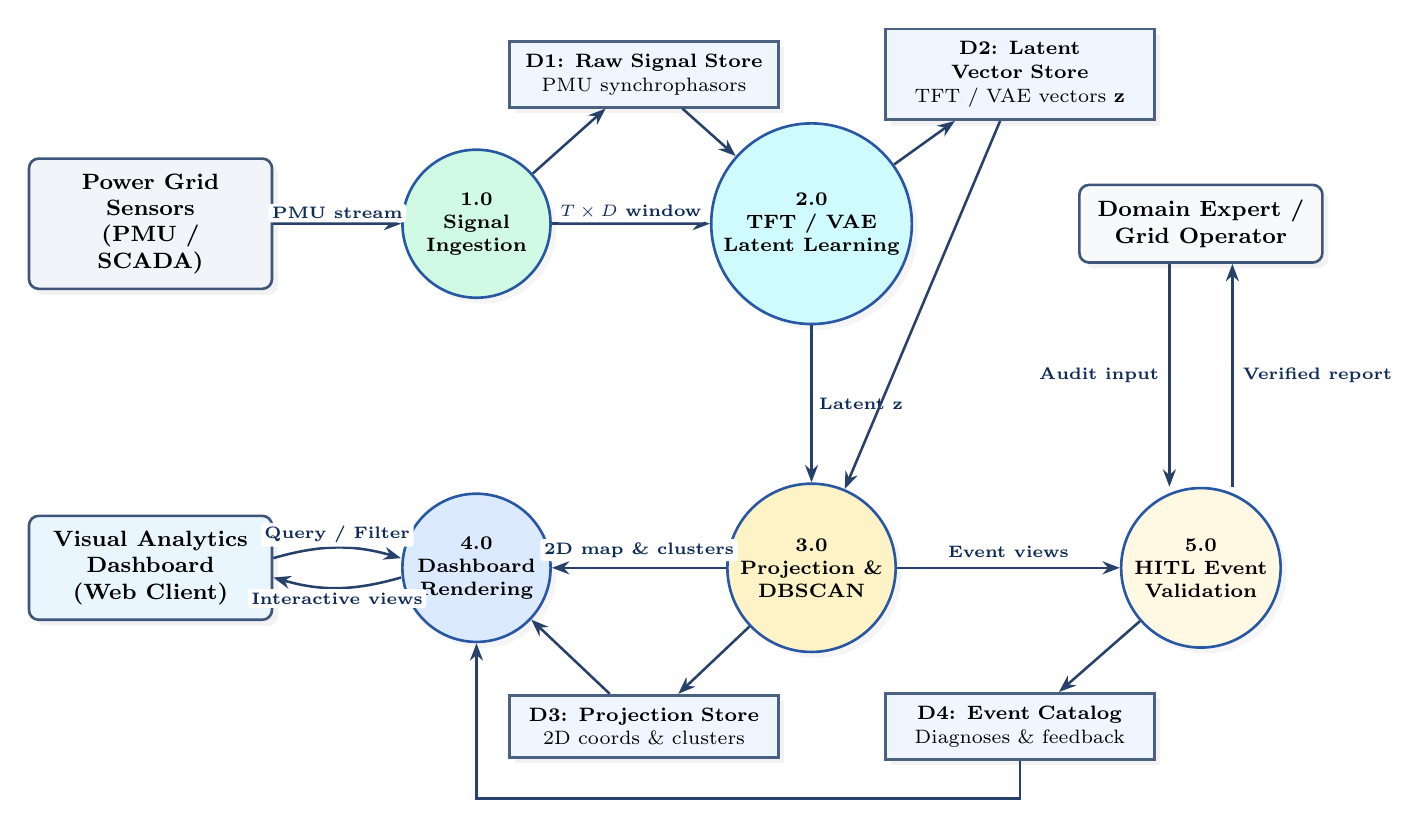
\begin{tikzpicture}[
  x=1.15cm, y=1.15cm,
  font=\sffamily,
  entity/.style={
    rectangle, draw=lavenderDark!80, line width=0.95pt, rounded corners=3.5pt,
    align=center, inner sep=5.5pt, font=\fontsize{8.0}{9.5}\selectfont\bfseries,
    text width=2.70cm, fill=cInput, drop shadow={opacity=0.10}
  },
  store/.style={
    rectangle, draw=lavenderDark!75, line width=0.95pt,
    align=center, inner sep=4.5pt, font=\fontsize{7.2}{8.6}\selectfont,
    text width=3.10cm, fill=lavenderLight, drop shadow={opacity=0.10}
  },
  proc/.style={
    circle, draw=lavenderMedium!95, line width=0.95pt,
    align=center, inner sep=2pt, minimum size=1.88cm,
    font=\fontsize{7.0}{8.3}\selectfont\bfseries, fill=cStage1, drop shadow={opacity=0.08}
  },
  procblue/.style={proc, fill=cStage4},
  procgold/.style={proc, fill=cStage2},
  prochead/.style={proc, fill=cHead},
  dfdarr/.style={
    -{Stealth[scale=0.88]}, line width=0.92pt, draw=lavenderDark!90
  },
  flowlbl/.style={
    font=\fontsize{6.0}{7.2}\selectfont\bfseries, fill=white, inner sep=1.3pt, text=lavenderDark, rounded corners=1pt
  }
]

  % External Entities
  \node[entity] (sensors) at (-5.8, 3.2) {Power Grid\\Sensors\\(PMU / SCADA)};
  \node[entity, fill=cStem!70] (ui) at (-5.8, -0.6) {Visual Analytics\\Dashboard\\(Web Client)};
  \node[entity, fill=cInput!60] (expert) at (5.8, 3.2) {Domain Expert /\\Grid Operator};

  % Processes
  \node[proc] (p1) at (-2.2, 3.2) {1.0\\Signal\\Ingestion};
  \node[procblue] (p2) at (1.5, 3.2) {2.0\\TFT / VAE\\Latent Learning};
  \node[procgold] (p3) at (1.5, -0.6) {3.0\\Projection \&\\DBSCAN};
  \node[prochead] (p4) at (-2.2, -0.6) {4.0\\Dashboard\\Rendering};
  \node[proc, fill=cStage2!50] (p5) at (5.8, -0.6) {5.0\\HITL Event\\Validation};

  % Data Stores (D1-D4 in standard quadrant order)
  \node[store] (d1) at (-0.35, 4.85) {\textbf{D1: Raw Signal Store}\\PMU synchrophasors};
  \node[store] (d2) at (3.8, 4.85) {\textbf{D2: Latent Vector Store}\\TFT / VAE vectors $\mathbf{z}$};
  \node[store] (d3) at (-0.35, -2.35) {\textbf{D3: Projection Store}\\2D coords \& clusters};
  \node[store] (d4) at (3.8, -2.35) {\textbf{D4: Event Catalog}\\Diagnoses \& feedback};

  % Data Flows - Top Row
  \draw[dfdarr] (sensors) -- node[above, flowlbl]{PMU stream} (p1);
  \draw[dfdarr] (p1) -- node[above, flowlbl]{$T \times D$ window} (p2);
  \draw[dfdarr] (p1) -- (d1);
  \draw[dfdarr] (d1) -- (p2);

  % Latent Flows
  \draw[dfdarr] (p2) -- node[right=1pt, flowlbl]{Latent $\mathbf{z}$} (p3);
  \draw[dfdarr] (p2) -- (d2);
  \draw[dfdarr] (d2) -- (p3);

  % Process 3.0 outputs (branching left to Dashboard, right to HITL)
  \draw[dfdarr] (p3) -- node[above=2pt, midway, flowlbl]{2D map \& clusters} (p4);
  \draw[dfdarr] (p3) -- (d3);
  \draw[dfdarr] (d3) -- (p4);
  \draw[dfdarr] (p3) -- node[above=2pt, midway, flowlbl]{Event views} (p5);

  % UI <-> Dashboard Rendering (Curved bidirectional paths with separated anchors)
  \draw[dfdarr] ([yshift=3.5pt]ui.east) to[bend left=16] node[above, flowlbl]{Query / Filter} ([yshift=3.5pt]p4.west);
  \draw[dfdarr] ([yshift=-3.5pt]p4.west) to[bend left=16] node[below, flowlbl]{Interactive views} ([yshift=-3.5pt]ui.east);

  % Domain Expert <-> HITL Validation (Separated parallel bidirectional flows)
  \draw[dfdarr] ([xshift=-0.40cm]expert.south) -- node[left=2pt, flowlbl]{Audit input} ([xshift=-0.40cm]p5.north);
  \draw[dfdarr] ([xshift=0.40cm]p5.north) -- node[right=2pt, flowlbl]{Verified report} ([xshift=0.40cm]expert.south);

  % HITL Feedback to Event Catalog & Dashboard
  \draw[dfdarr] (p5) -- (d4);
  \draw[dfdarr] (d4.south) -- ++(0, -0.42) -| (p4.south);

\end{tikzpicture}
\end{document}
